\chapter{Formatierungsbeispiele}

Formatierungsbeispiele

vgl. Abbildung~\ref{fig:beispiel}

\begin{figure}[ht]
  \centering
  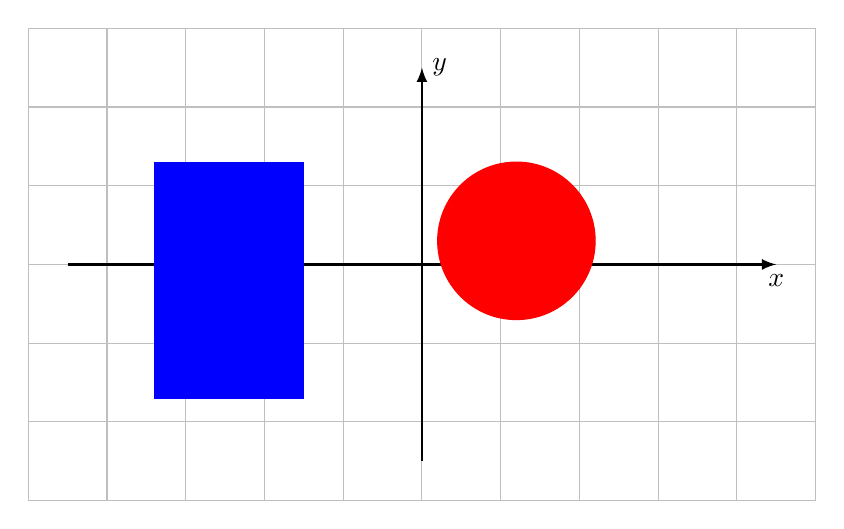
\begin{tikzpicture}
    \draw[draw=lightgray, step=1cm] (-5, -3) grid (5, 3);
    \draw[thick, -latex] (-4.5, 0) -- (4.5, 0) node[below] {$x$};
    \draw[thick, -latex] (0, -2.5) -- (0, 2.5) node[right] {$y$};
    \draw[draw=red, fill=red] (1.2, 0.3) circle (1cm);
    \draw[draw=blue, fill=blue] (-3.4, -1.7) rectangle (-1.5, 1.3);
  \end{tikzpicture}
  \caption{Ein Beispielbild, natürlich mit Bildunterschrift.}
  \label{fig:beispiel}
\end{figure}




\begin{align}
  \sin(x+2\pi) &= \sin(x)\\
  \cos(x+2\pi) &= \cos(x)\\
  \cos(x) &= \sin\left(x+\frac{\pi}{2}\right)
\end{align}


\section{Section}

\begin{table}
  \centering
  \begin{tabular}{l|c|r}
	links & mittig & rechts\\\hline
	a & b & c\\
	1 & 2 & 3  
  \end{tabular}
  \caption{Eine Beispieltabelle, natürlich mit einer Erläuterung.}
  \label{tab:beispiel}
\end{table}
